\chapter{Optimisation Strategy} \label{chp:opt-strategy}

Although the technique proposed in Chapter~ref{chp:fm-operation} is able to merge any two functions, it is not always profitable to do so.
In fact, as it is only profitable to merge functions that are sufficiently similar, for most pairs of functions, merging them increases code size.
Therefore, we must be able to decide which merge operations are profitable.
%Therefore, we must be able to decide which pairs of functions are most likely to be profitably merged.

\section{Profitability Analysis}\label{sec:profit-model}

A merge operation is profitable when replacing the original pair of functions by the merged function results in an overall smaller code.
Since merging most pairs of functions tend to produce a much larger function, the profitability analysis is critical for the optimisation strategy.

In order to estimate the code-size benefit, we first estimate the size of all three functions.
The size of each function is estimated by summing up the estimated binary size of all instruction in the function.
The binary size of each instruction is estimated by querying the compiler's built-in target-specific cost model.
As described in Section~\ref{sec:background:costmodel}, although the cost model estimations are not necessarily precise, they are useful for comparing two pieces of code and deciding when a replacement is profitable.

% The actual cost of each instruction comes from querying this compiler's built-in cost model, which provides a target-dependent cost estimation that approximates the code-size cost of an IR instruction when lowered to machine instructions.

In addition to measuring the difference in size of the merged function, we also need to take into account all extra costs involved in replacing the original functions with the merged one:
$(1)$ for the cases where we need to keep a \textit{thunk} of the original functions, preserving their original signatures; % with a call to the merged function;
and $(2)$ for the cases where we update the call graph, there might be an extra cost with a call to the merged function due to the increased number of arguments.

Let $c(f)$ be the code-size cost of a given function $f$, and
$\delta(f_i, f_j)$ represent the extra costs involved when replacing or
updating function $f_i$ with the function $f_j$.
Therefore, given a pair of functions $\{f_1,f_2\}$ and the merged function
$f_{1,2}$, we want to maximise the profit defined as:
\[
  \Delta(\{f_1,f_2\},f_{1,2}) = (c(f_1)+c(f_2)) - (c(f_{1,2}) + \varepsilon)
\]
where $\varepsilon = \delta(f_1, f_{1,2}) + \delta(f_2, f_{1,2})$.
We consider that the merge operation is profitable if $\Delta(\{f_1,f_2\},f_{1,2})>0$.

However, these cost models are expected to contain inaccuracies.
Because we are operating on the IR level, one IR instruction does not necessarily translate to one machine instruction.
Several number of optimisations and code transformations will run afterwards, modifying the code.
Moreover, we cannot know exactly how each IR instruction will be lowered without actually running the compiler's backend.
The same IR instruction can be lowered to different machine instructions, depending on its surrounding context, the instruction selection algorithm, and many other factors.
Therefore, there is also an inherent limitation of estimating the cost of each instruction separately of its context.
However, the use of cost models is still a good trade-off between compilation time and accuracy.
%% TODO: Cite the Ithemal paper and add more text.

%Even though statically estimating code-size cost of an instruction is easier than the performance cost.
% sources of inaccuracies: IR level, many optimisations will run afterwards, which means that some instructions might be removed, replaced or added.
% At the IR level, we cannot know exactly how each IR instruction will be lowered, the same IR instruction can be lowered to different machine instructions, depending on the surrounding context, the instruction selection algorithm, etc. Therefore, we are limited by estimating the cost of each instruction separately of its context.
%Because of that, the profitability is measured with the help of the compiler's target-specific cost model.
%The actual cost of each instruction comes from querying this compiler's built-in cost model, which provides a target-dependent cost estimation that approximates the code-size cost of an IR instruction when lowered to machine instructions.
% However, the use of cost models is still a good trade-off between compilation time and accuracy. Cite the Ithemal paper and add more text.
%Our implementation makes use of the code-size costs provided by LLVM's target-transformation interface (TTI), which is widely used in the decision making of most optimisations~\cite{porpodas18b,pohl18}.

\section{Exhaustive Search}


\section{Focusing on Profitable Functions}
\label{sec:framework}

%In this section, we describe our implementation of the function merging
%optimisation, which combines the proposed function-merging technique with an
%efficient exploration infrastructure.

%In this section, we describe our exploration infrastructure for the
%function merging optimisation.

In this section, we introduce our framework for efficiently exploring the
optimisation space, focusing on pairs of functions that are profitable to merge. 

%Therefore,
%the main goal of our exploration infrastructure is to efficiently find pairs of functions that are profitable to merge.
%%
%As described in Section~\ref{sec:background}, LLVM's existing function merging
%optimisation, due to its hard restriction of only merging identical functions,
%is able to  efficiently explore which functions to merge by computing a hash
%of the functions.
%If two functions have the same hash, they are very likely to be identical.
%Moreover, merging identical functions is always profitable.
%For the proposed function-merging technique, on the other hand, because it is
%able to merge any pair of functions, we have a much larger exploration space and
%also a more challenging decision problem.

%\subsection{Ranking Infrastructure}

For every function, ideally, we would like to try to merge it with all other functions and choose the pair that maximises the reduction in code size.
However, this quadratic exploration over all pairs of functions results in prohibitively expensive compilation overhead.
In order to avoid the quadratic exploration of all possible merges, we propose the exploration framework shown in Figure~\ref{fig:func-merge-opt-arch} for our optimisation.
\begin{figure}[t!]
  \centering
  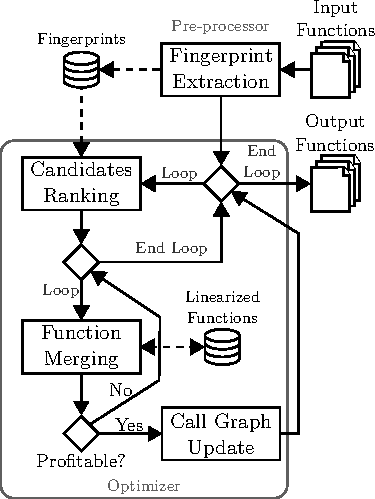
\includegraphics[width=0.7\linewidth]{src/merging-optimisation/figs/func-merge-opt-arch.pdf}
  \caption{Overview of our exploration framework.}
  \label{fig:func-merge-opt-arch}
\end{figure}

The proposed framework is based on a light-weight ranking infrastructure that uses a \textit{fingerprint} of the functions to evaluate
their similarity. It starts by precomputing and caching fingerprints for all functions. The purpose of fingerprints is to make it easy
to discard unpromising pairs of functions so that we perform the more expensive evaluation only on the most promising pairs.
To this end, the fingerprint consists of: $(1)$ a map of instruction opcodes to their frequency in the function; $(2)$ the set of types
manipulated by the function. While functions can have several thousands of instructions, an IR usually has just a few tens of opcodes,
e.g., the LLVM IR has only about 64 different opcodes. This means that the fingerprint needs to store just a small integer array of the
opcode frequencies and a set of types, which allows for an efficient similarity comparison.

By comparing the opcode frequencies of two functions, we are able to estimate
the best case merge, which would happen if all instructions with the same opcode could match.
This is a very optimistic estimation. It would be possible only if instruction types and order
did not matter. We refine it further by estimating another best case merge, this time based
on type frequencies, which would happen if all instructions with the same data type could match.


%This assumption provides an upper bound on the actual number of matches, since
%it may be affected by the instruction types and the order they appear in the
%linearised functions.
%As a way to refine this estimate, we weight this upper bound by the Jaccard
%similarity coefficient~\cite{jaccard} of the sets of types, i.e., a
%type-similarity ratio between the two functions.
%Formally, let $T_1$ and $T_2$ be the set of types of the functions $f_1$ and
%$f_2$, respectively.
%In order to refine this upper-bound estimate, we also compare the type frequencies
%of the two functions, this time assuming that all instructions with the same
%data type would always result in a match.
Therefore, the upper-bound reduction, computed as a ratio, can be generally defined as
%\[
%   U\!B(f_1,f_2) = \frac{\sum\limits_{op \in Ops} \min\{freq(op,f_1),freq(op,f_2)\}}{\sum\limits_{op \in Ops} freq(op,f_1)+freq(op,f_2)}
%\]
\[
   U\!B(f_1,f_2, K) = \frac{\sum\limits_{k \in K} \min\{freq(k,f_1),freq(k,f_2)\}}{\sum\limits_{k \in K} freq(k,f_1)+freq(k,f_2)}
\]
where $U\!B(f_1,f_2, Opcodes)$ computes the opcode-based upper bound and
$U\!B(f_1,f_2, Types)$ computes the type-based upper bound.
The final estimate selects the minimum upper bound between the two, i.e.,
\[
%     s(f_1,f_2) = U\!B(f_1,f_2) \frac{|T_1 \cap T_2|}{|T_1 \cup T_2|}.
     s(f_1,f_2) = \min\{U\!B(f_1,f_2, Opcodes), U\!B(f_1,f_2, Types)\}
\]
This estimate results in a value in the range $[0,0.5]$,
which encodes a description that favours maximizing both the opcode and type
similarities, while also minimizing their respective differences.
Identical functions will always result in the maximum value of $0.5$.

For each function $f_1$, we use a priority queue to rank the topmost
similar candidates based on their similarity, defined by $s(f_1,f_2)$, for all
other functions $f_2$.
We use an exploration threshold to limit how many top candidates we will
evaluate for any given function.
We then perform this candidate exploration in a greedy fashion, terminating after
finding the first candidate that results in a profitable merge and committing that
merge operation.

\begin{figure}[t!]
  \centering
  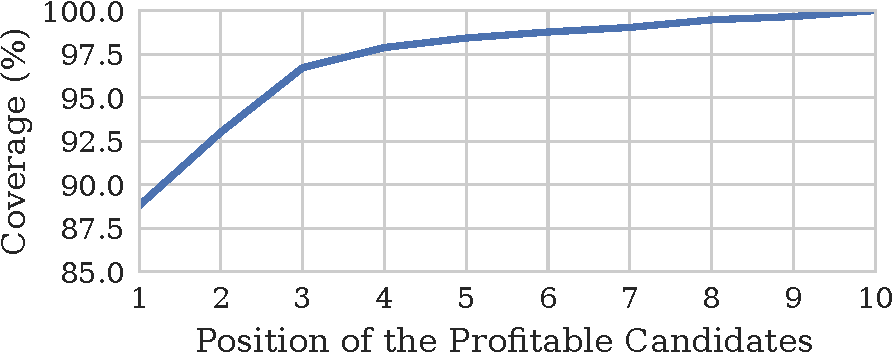
\includegraphics[width=0.8\linewidth]{src/merging-optimisation/figs/average-cdf-exploration-threshold.pdf}
  \caption{Average CDF for the position of the profitable candidate and the percentage of merged operations covered.
           %Average CDF for the exploration threshold and the percentage of merged operations covered.
           89\% of the merge operations happen with the topmost candidate.}
           %A merge operation happens with the topmost candidate in about 89\% of the cases.}
  \label{fig:average-cdf-exploration-threshold}
\end{figure}

Ideally, profitable candidates will be as close to the top of the rank as
possible.
Figure~\ref{fig:average-cdf-exploration-threshold} shows the cumulative
distribution of the position of the profitable candidates in a top 10 rank.
It shows that about 89\% of the merge operations occurred with the topmost
candidate, while the top 5 cover over 98\% of the profitable candidates.
These results suggest that fingerprint similarity is able to
accurately capture the real function similarity, while reducing the exploration
cost by orders of magnitudes, depending on the actual number and size of
the functions.

When a profitable candidate is found, we first replace the body of the two
original functions to a single call to the merged function.
Afterwards, if the original functions can be completely removed, we update the
call graph, replacing the calls to the original functions by calls to the
merged function.
Finally, the new function is added to the optimisation working list.
Because of this feedback loop, merge operations can also be performed on
functions that resulted from previous merge operations.

\section{Placement of the Optimisation}

There are different ways of applying this optimisation, with different trade-offs.
We can apply our optimisation on a per compilation-unit basis, which usually
results in lower compilation-time overheads because only a small part of the
whole program is being considered at each moment.
However, this also limits the optimisation opportunities, since only pairs of
functions within the same translation unit would be merged.

On the other hand, our optimisation can also be applied in the whole program,
for example, during link-time optimisation (LTO).
Optimizing the whole program is beneficial for the simple fact that the
optimisation will have more functions at its disposal.
It allows us to merge functions across modules.

\begin{figure}[h]
  \centering
  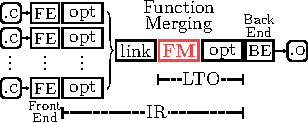
\includegraphics[width=0.7\linewidth]{src/merging-optimisation/figs/opt-pipeline.pdf}
  \caption{In our experiments we use a compilation pipeline with a monolithic link-time optimisation (LTO).}
  \label{fig:opt-pipeline}
\end{figure}


In addition to the benefit of being able to merge more functions, when optimizing
the whole program, we can also be more aggressive when removing the original functions,
since we know that there will be no external reference to them.
However, if the optimisation is applied per translation unit, then extra
conditions must be guaranteed, e.g., the function must be explicitly defined
as internal or private to the translation unit.

\section{Evaluation}

In this section, we evaluate the proposed optimization, where we analyze our
improvements on code size reduction, as well as its impact on the program's
performance and compilation-time.

\subsection{Code-Size Reduction}

Figure~\ref{fig:reduction-obj} reports the code size reduction over the baseline for the linked object. %These results show how much we can improve over the existing techniques, by having a more powerful solution, and how close we
%can get to the oracle with our ranking-based exploration framework.
We observe similar trends of code size reduction on both target architectures. This is expected because the
optimizations are applied at the platform-independent IR level. Changing the target architecture introduces only second order effects,
such as slightly different decisions due to the different cost model (LLVM's TTI) and differences in how the IR is encoded into binary.

\begin{figure*}[h]
  \centering
  %\includegraphics[width=\linewidth]{figs/reduction-obj-intel-label.pdf} \\
  %\includegraphics[width=\linewidth]{figs/reduction-obj-arm-label.pdf}
  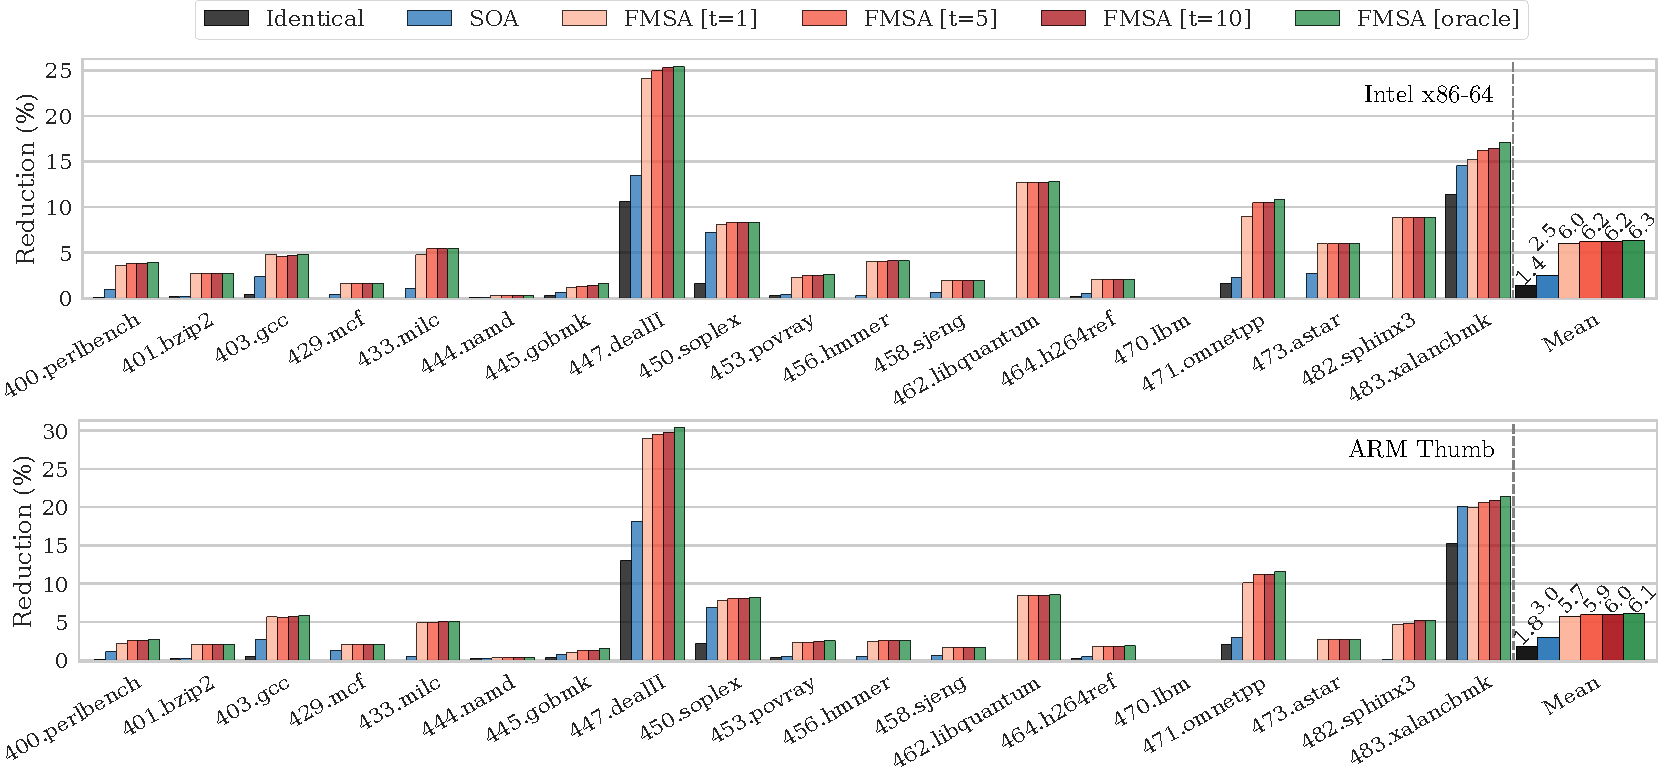
\includegraphics[width=\linewidth]{src/merging-optimisation/figs/code-size-reduction-spec.pdf}
	\caption{Object file size reduction for Intel (top) and ARM (bottom). We evaluate our approach (FMSA) under four different exploration thresholds, which
      control how many potential merging pairs we examine for each function before making a decision. Even for a threshold of one, we outperform the state-of-the-art
	  by 2.4$\times$~(Intel) and 1.9$\times$~(ARM).}
  \label{fig:reduction-obj}
\end{figure*}

Our approach, FMSA, significantly improves over the state-of-the art (SOA). For the Intel platform, FMSA can achieve an average code size
reduction of up to 6.3\% (or 6\% with the lowest exploration threshold), while the SOA and Identical had an average reduction of 2.5\% and 1.4\%,
respectively. Similarly, for the ARM platform, FMSA can achieve an average code size reduction of up to 6.1\% (or 5.7\% with the lowest
threshold), while SOA and Identical had an average reduction of 3\% and 1.8\%, respectively. For several of the benchmarks, the
proposed technique achieves impressive code size reduction compared to other merging approaches.


In most cases, LLVM's identical function merging has very little impact on code
size.
We see noticeable impact only on some of the C++ benchmarks, namely,
\texttt{447.dealII}, \texttt{450.soplex}, \texttt{471.omnetpp}, \texttt{483.xalancbmk}.
These are the cases that identical function merging was designed to handle,
duplicate functions due to heavy use of templating.
%But even on these benchmarks FMSA outperforms LLVM, with an improvement of
%almost 6$\times$ on \texttt{471.omnetpp}.
Although the state-of-the-art improves over LLVM's identical function merging,
it still gets most of its code size reduction for benchmarks with heavy use of templating.
In addition to achieving better results in all of these cases, our technique
%On the other hand, FMSA is able to achieve better results in all these cases.
%FMSA is designed to merge a superset of the functions that the LLVM identical
%function merging can handle while having much less restrictions than the
%state-of-the-art, so it is able to achieve better results in all these cases.
%Moreover, our technique
also shows remarkable reductions on several of the
C benchmarks, especially \texttt{462.libquantum} and \texttt{482.sphinx3}, where
other techniques have no real impact.


In Section~\ref{sec:motivation}, we show two examples extracted from
\texttt{462.libquantum} and \texttt{482.sphinx3}, where we detail how existing
techniques fail to merge similar functions in these benchmarks.
Our technique is the \textit{first} that can handle these examples, producing
merged functions equivalent to the handwritten ones shown in
Figures~\ref{fig:sphinx-example} and~\ref{fig:libquantum-example}.


\begin{table}[h]
\centering
\caption{Number and size of functions present in each SPEC CPU2006 benchmark just before function merging, as well as number of merge operations applied by each technique.}
\scalebox{0.71}{
\begin{tabular}{lllllll}
\toprule
\multicolumn{1}{c}{\textbf{Benchmarks}} & \textbf{\#Fns} & \textbf{Min/Avg/Max Size} &\textbf{Identical} & \textbf{SOA}  & \textbf{FMSA{[}t=1{]}} & \textbf{FMSA{[}t=10{]}} \\
\midrule
                     400.perlbench      & 1699   & 1 / 125 / 12501    & \small 12     & \small 103   & \small 175  & \small 200  \\
\rowcolor{evencolor} 401.bzip2          & 74     & 1 / 206 / 5997     & \small 0      & \small 0     & \small 7    & \small 7    \\
                     403.gcc            & 4541   & 1 / 127.7 / 20688  & \small 136    & \small 341   & \small 614  & \small 710  \\
\rowcolor{evencolor} 429.mcf            & 24     & 18 / 87.25 / 297   & \small 0      & \small 1     & \small 1    & \small 1    \\
                     433.milc           & 235    & 1 / 67.69 / 416    & \small 0      & \small 6     & \small 26   & \small 34   \\
\rowcolor{evencolor} 444.namd           & 99     & 1 / 570.64 / 1698  & \small 1      & \small 1     & \small 5    & \small 5    \\
                     445.gobmk          & 2511   & 1 / 43.22 / 3140   & \small 183    & \small 485   & \small 436  & \small 605  \\
\rowcolor{evencolor} 447.dealII         & 7380   & 1 / 60.63 / 4856   & \small 1835   & \small 2785  & \small 2974 & \small 3315 \\
                     450.soplex         & 1035   & 1 / 73.27 / 1719   & \small 27     & \small 125   & \small 156  & \small 163  \\
\rowcolor{evencolor} 453.povray         & 1585   & 1 / 98.05 / 5324   & \small 60     & \small 112   & \small 193  & \small 212  \\
                     456.hmmer          & 487    & 1 / 99.98 / 1511   & \small 3      & \small 16    & \small 45   & \small 47   \\
\rowcolor{evencolor} 458.sjeng          & 134    & 1 / 145.06 / 1252  & \small 0      & \small 5     & \small 11   & \small 11   \\
                     462.libquantum     & 95     & 1 / 56.64 / 626    & \small 0      & \small 1     & \small 9    & \small 9    \\
\rowcolor{evencolor} 464.h264ref        & 523    & 1 / 171.42 / 5445  & \small 3      & \small 22    & \small 50   & \small 52   \\
                     470.lbm            & 17     & 6 / 123.41 / 680   & \small 0      & \small 0     & \small 0    & \small 0    \\
\rowcolor{evencolor} 471.omnetpp        & 1406   & 1 / 26.9 / 611     & \small 45     & \small 69    & \small 227  & \small 270  \\
                     473.astar          & 101    & 1 / 67.11 / 584    & \small 0      & \small 2     & \small 4    & \small 4    \\
\rowcolor{evencolor} 482.sphinx3        & 326    & 1 / 80 / 924       & \small 2      & \small 6     & \small 24   & \small 26   \\
                     483.xalancbmk      & 14191  & 1 / 38.58 / 3809   & \small 3057   & \small 4573  & \small 4342 & \small 4887 \\
\bottomrule
\end{tabular}
}
\label{tab:stats}
\end{table}

Table~\ref{tab:stats} provides detailed statistics for the SPEC CPU2006.
We show how many functions (\#Fns) are present in the linked program
just before the merging pass, as well as
the average, minimum, and maximum size of these functions, in number of instructions, at
this same point in the compilation pipeline.
We also report how many pair-wise merge operations are
performed by each one of the function merging techniques.
Note that in almost all cases FMSA performs significantly more merge operations than the other
techniques.
There are only two cases where FMSA with exploration threshold of one finds fewer
profitable merges than the state-of-the-art. This is due to our aggressive pruning
of the search space with our ranking mechanism. Simply increasing the threshold, e.g. to ten,
allows FMSA to merge more functions. In any case, these extra merge operations of the state-of-the-art
have little effect on the overall code size reduction. The state-of-the-art is more likely to fail to
merge large functions and succeed with small ones, so even when merging more functions, it does not
reduce code size as much as FMSA.

\subsubsection*{MiBench: Embedded Benchmark Suite}

We have shown that our technique achieves good results when applied on the SPEC
CPU suite. It reduces size not only on templated C++ benchmarks, like other
techniques, but also on C benchmarks where merging opportunities should
be almost non-existant. Here, we further explore how FMSA handles such
cases by applying it on the MiBench suite, a collection of small C programs
each one composed of a small number of functions. 

Figure~\ref{fig:code-size-reduction-mibench} shows the object file reduction
for the MiBench programs on the Intel platform. Our best result is for the \texttt{rijndael} benchmark,
which implements the well-known AES encryption. FMSA merges the two largest functions, namely,
\texttt{encrypt} and \texttt{decrypt}.
Inspecting the LLVM IR for the \texttt{rijndael} benchmark, we observe that
the two functions contain a total of 2494 instructions, over 70\% of the code.
When we merge them by sequence alignment, we create a single function with
only 1445 instruction, a 42\% reduction in the number of IR instructions. This
translates into a 20.6\% reduction in the linked object file.

\begin{table}[h]
\centering
\caption{Number and size of functions present in each MiBench benchmark just before function merging, as well as number of merge operations applied by each technique.}
\scalebox{0.75}{
\begin{tabular}{lllllll}
\toprule
\multicolumn{1}{c}{\textbf{Benchmarks}} & \textbf{\#Fns} & \textbf{Min/Avg/Max Size} &\textbf{Identical} & \textbf{SOA}  & \textbf{FMSA{[}t=1{]}}  & \textbf{FMSA{[}t=10{]}} \\
\midrule
                     CRC32         & 4     & 8 / 24.75 / 39       & \small 0     & \small 0   & \small 0    & \small 0   \\
\rowcolor{evencolor} FFT           & 7     & 7 / 49.86 / 144      & \small 0     & \small 0   & \small 0    & \small 0   \\
                     adpcm\_c      & 3     & 37 / 73 / 100        & \small 0     & \small 0   & \small 0    & \small 0   \\
\rowcolor{evencolor} adpcm\_d      & 3     & 37 / 73 / 100        & \small 0     & \small 0   & \small 0    & \small 0   \\
                     basicmath     & 5     & 4 / 70.8 / 232       & \small 0     & \small 0   & \small 0    & \small 0   \\
\rowcolor{evencolor} bitcount      & 19    & 4 / 22.26 / 63       & \small 0     & \small 1   & \small 3    & \small 3   \\
                     blowfish\_d   & 8     & 1 / 245.38 / 824     & \small 0     & \small 0   & \small 0    & \small 0   \\
\rowcolor{evencolor} blowfish\_e   & 8     & 1 / 245.38 / 824     & \small 0     & \small 0   & \small 0    & \small 0   \\
                     jpeg\_c       & 322   & 1 / 100.52 / 1269    & \small 2     & \small 6   & \small 8    & \small 11  \\
\rowcolor{evencolor} jpeg\_d       & 310   & 1 / 98.93 / 1269     & \small 3     & \small 6   & \small 10   & \small 10  \\
                     dijkstra      & 6     & 2 / 33 / 89          & \small 0     & \small 0   & \small 0    & \small 0   \\
\rowcolor{evencolor} ghostscript   & 3446  & 1 / 54.2 / 4218      & \small 53    & \small 53  & \small 234  & \small 250 \\
                     gsm           & 69    & 1 / 97.06 / 737      & \small 0     & \small 3   & \small 8    & \small 8   \\
\rowcolor{evencolor} ispell        & 84    & 1 / 105.51 / 1082    & \small 0     & \small 2   & \small 5    & \small 5   \\
                     patricia      & 5     & 1 / 77 / 167         & \small 0     & \small 0   & \small 0    & \small 0   \\
\rowcolor{evencolor} pgp           & 310   & 1 / 88.52 / 1845     & \small 0     & \small 1   & \small 10   & \small 10  \\
                     qsort         & 2     & 11 / 50 / 89         & \small 0     & \small 0   & \small 0    & \small 0   \\
\rowcolor{evencolor} rijndael      & 7     & 46 / 472.29 / 1247   & \small 0     & \small 0   & \small 1    & \small 1   \\
                     rsynth        & 46    & 1 / 97.28 / 778      & \small 0     & \small 0   & \small 0    & \small 0   \\
\rowcolor{evencolor} sha           & 7     & 12 / 53.29 / 150     & \small 0     & \small 0   & \small 0    & \small 0   \\
                     stringsearch  & 10    & 3 / 47.9 / 99        & \small 0     & \small 0   & \small 1    & \small 1   \\
\rowcolor{evencolor} susan         & 19    & 15 / 291.84 / 1212   & \small 0     & \small 0   & \small 1    & \small 1   \\
                     typeset       & 362   & 1 / 354.47 / 12125   & \small 1     & \small 4   & \small 31   & \small 35  \\
\bottomrule
\end{tabular}
}
\label{tab:stats-mibench}
\end{table}


\begin{figure*}[t]
  \centering
  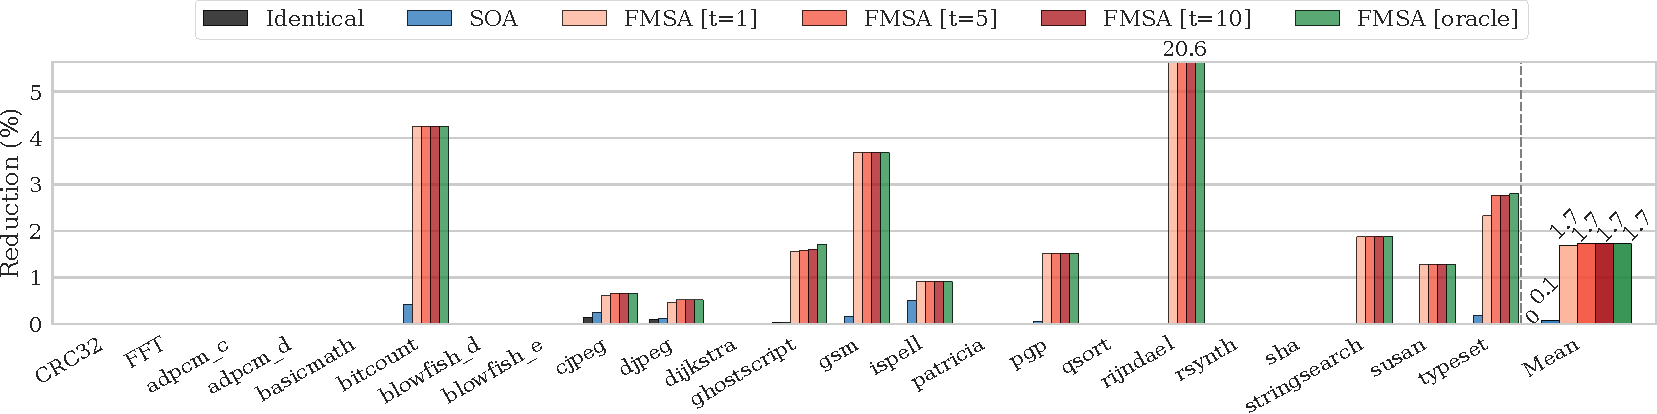
\includegraphics[width=\linewidth]{src/merging-optimisation/figs/code-size-reduction-mibench.pdf}
  \caption{Object file size reduction for Intel on the Mibench benchmark suite.
   Our approach (FMSA) is the only one able to achieve a meaningful reduction on these benchmarks.
   }
  \label{fig:code-size-reduction-mibench}
\end{figure*}

Table~\ref{tab:stats-mibench} provides more detailed statistics for MiBench.
LLVM achieves very limited results, reducing \texttt{jpeg\_c} by just 0.13\%,
\texttt{jpeg\_d} by 0.1\%, and \texttt{ghostscript} by 0.02\%, while having no effect on \texttt{typeset}.
This happens because all the functions merged by LLVM's identical technique are tiny functions relative to the overall size of the program.
Most of these functions comprise of just a few IR instructions. For example, in the \texttt{typeset} benchmark,
while it is able to merge a pair of functions, they only have five instructions. For the same benchmark, FMSA performs several merge operations, one of them between two functions with over 500 instructions.
Overall, the state-of-the-art does slightly better than LLVM's identical technique but even in its best case it cannot reduce code size more than 0.7\%.

Because these embedded benchmarks are much smaller than those in the SPEC suite, trivially similar functions are much less frequent.
This is why neither the state-of-the-art nor LLVM's identical function merging technique had any real effect on these benchmarks.
Our technique can look beyond trivially similar functions which allowed it to achieve significant code size reduction on these real embedded benchmarks.

\subsection{Compilation Overhead}

Figure~\ref{fig:compilation-time} shows the compilation-time overhead for all optimizations. As explained in the experimental setup, we
only present results when compiling for the Intel platform. Since we cross-compile on the same machine for both targets, compilation times
are very similar. We also do not include results for the oracle (exhaustive) exploration. It would be hard to visualize it in the same plot
as the other configurations, since it can be up to 136$\times$ slower than the baseline.

\begin{figure*}[t]
  \centering
  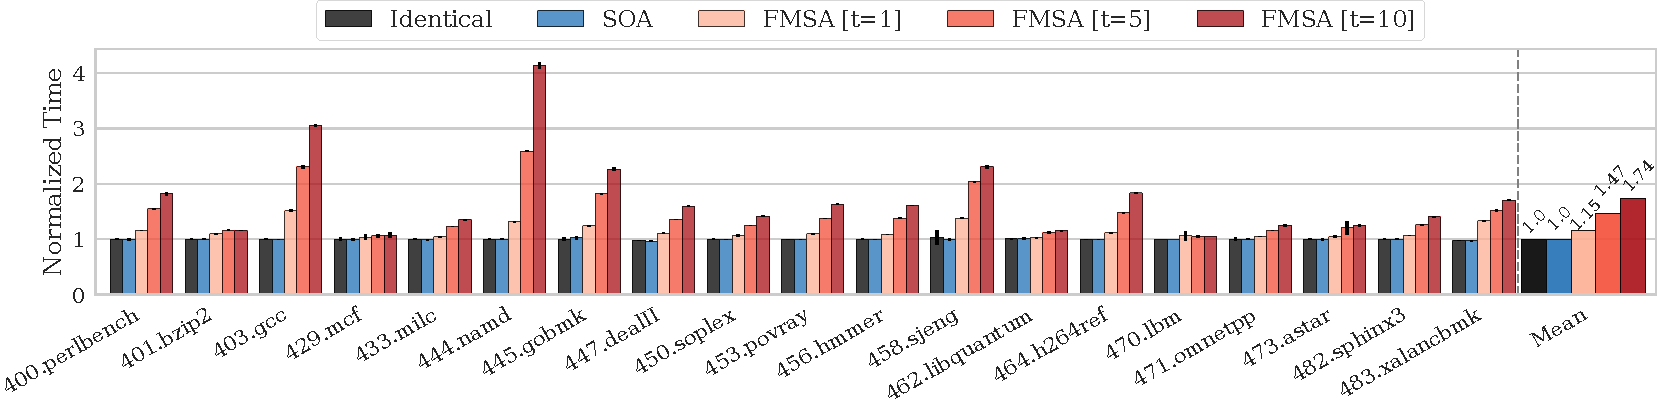
\includegraphics[width=\linewidth]{src/merging-optimisation/figs/compilation-time.pdf}
	\caption{Compilation-time overhead on the Intel platform. For exhaustive exploration (not shown) the average overhead is 25$\times$. Through ranking, we reduce overhead by orders of magnitude. For an exploration threshold of one, FMSA has an overhead of only 15\%.}
  \label{fig:compilation-time}
\end{figure*}

Unlike the other evaluated techniques, our optimization is a prototype implementation, not yet tuned for compilation-time. We believe that
compilation-time can be further reduced with some additional engineering effort. Nevertheless, by using our ranking infrastructure to
target only the single most promising equivalent function for each function we examine, we reduce compilation-time overhead by up to two
orders of magnitude compared to the oracle. This brings the average compile-time overhead to only 15\% compared to the baseline, while
still reducing code size almost as well as the oracle. Depending on the acceptable trade-off between compilation-time overhead and code
size, the developer can change the exploration threshold to exploit more opportunities for code reduction, or to accelerate compilation.

\begin{figure}[h]
  \centering
  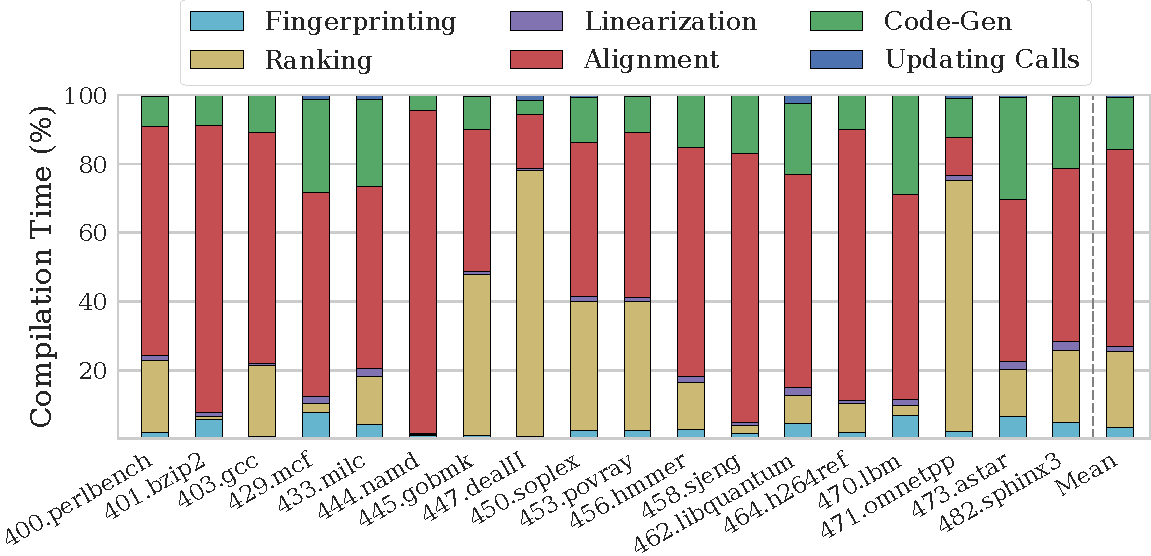
\includegraphics[width=1.0\linewidth]{src/merging-optimisation/figs/compilation-time-breakdown-sqrd.pdf}
  \caption{A compilation-time breakdown isolating the percentage for each major
           step of the optimization (t=1).}%, with an exploration threshold of one.}
  \label{fig:compilation-time-breakdown}
\end{figure}


Figure~\ref{fig:compilation-time-breakdown} shows a detailed compilation-time breakdown. For each major step of the proposed optimization,
we present the accumulated time spent across the whole program. To better understand the overhead of each step, we use an exploration threshold of one ($t = 1$). Because the ranking mechanism performs a quadratic operation on the number of functions, computing
the similarity between all pairs of functions, it is expected that ranking would be amongst the most costly steps. However, it is
interesting to notice that the sequence alignment dominates most of the compilation-time overhead, especially considering that this
operation is performed only once per function, when $t = 1$. Although this operation is linear in the number of functions, the
Needleman-Wunsh algorithm~\cite{needleman70} is quadratic in the size of the functions being aligned, both in time and space.
Unsurprisingly, code generation is the third most costly step, which also includes the time to optimize the merge of the parameters. The
remaining steps contribute, in total, a small percentage of all the compilation-time overhead. This analysis suggests that optimizing the
sequence alignment algorithm and the ranking mechanism is key to reducing even further the overall compilation-time overhead.

\subsection{Performance Impact}

The primary goal of function merging is to reduce code size. Nevertheless, it is also important to understand its impact on the programs'
execution time and the trade-offs between performance and code size reduction. Figure~\ref{fig:runtime-impact} shows the normalized
execution time. Overall, our optimization has an average impact of about 3\% on programs' runtime. For most benchmarks, there is no
statistically significant difference between the baseline and the optimized binary. Only for \texttt{433.milc}, \texttt{447.dealII}, and
\texttt{464.h264ref} there is a noticeable performance impact.

\begin{figure*}[h]
  \centering
  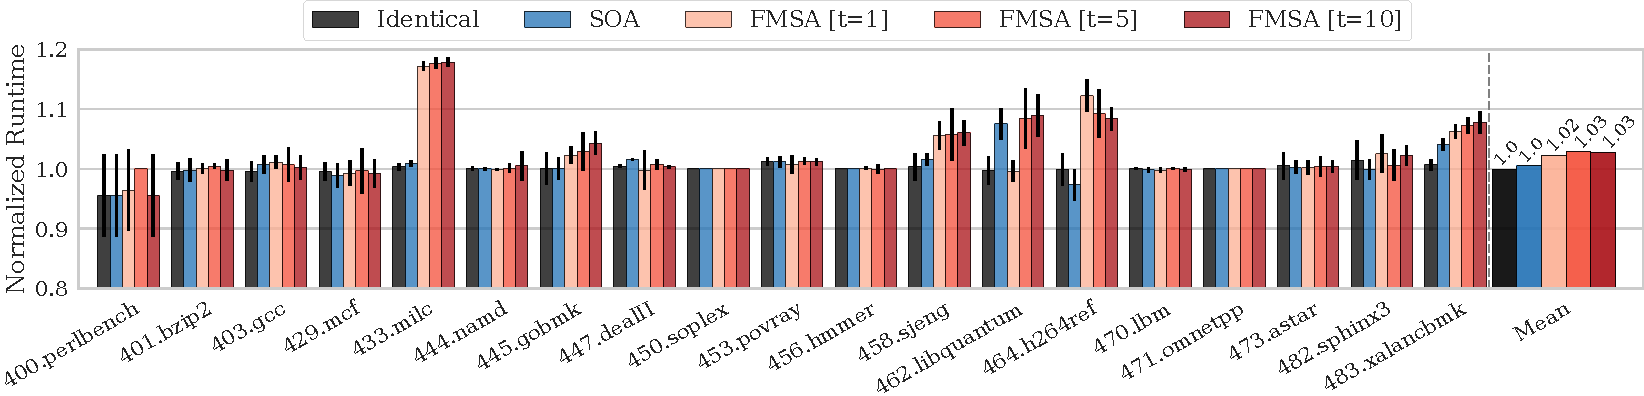
\includegraphics[width=\linewidth]{src/merging-optimisation/figs/runtime-impact.pdf}
  \caption{Runtime overhead on the Intel platform. Performance impact is almost always statistically insignificant. For the few benchmarks affected, FMSA merges hot functions.}
  \label{fig:runtime-impact}
\end{figure*}

%\begin{figure}[t]
%  \centering
%  \includegraphics[width=0.8\linewidth]{figs/profiling-results.pdf}
%  \caption{Profile-guided function merging on the \texttt{433.milc} benchmark.}
%  \label{fig:pgo-results}
%\end{figure}

We take \texttt{433.milc}, which has the worst result, for discussion. For an exploration threshold value of one, we merge 58 functions.
Through profiling, we discovered that a handful of them contain hot code, that is, they have basic blocks that are frequently executed. If we prevent these hot
functions from merging, all performance impact is removed while still reducing code size. Specifically, our original results showed a
5.11\% code size reduction and an 18\% performance overhead.
Avoiding merging hot functions results in effectively non-existent performance impact and
a code size reduction of 2.09\%.
This code size reduction is still about twice as good as the state-of-the-art. As with the
compilation overhead, this is a trade-off that the developer can control.
